\documentclass[compress]{beamer}
\usepackage{graphics}
\usepackage{hyperref}
\hypersetup{
    colorlinks,
    citecolor=blue,
    filecolor=black,
    linkcolor=blue,
    urlcolor=blue,
    bookmarksopen = false,
    %pdfstartview = {XYZ null null 1.00}
 	%pdfpagemode=None
}
\usepackage{amsmath}
\usepackage{beamerthemesplit}
\usepackage{multicol}
\usetheme[hoptionsi]{Madrid}
%\usetheme{CambridgeUS}
\useinnertheme{rectangles}
%\usecolortheme{dolphin}
 \title[Masters Dissertation]{Masters Dissertation}
 \subtitle {``Smart Cafeteria'' Adaptive And Interactive Mobile Application}
 \logo{%
    
\includegraphics[width=1cm,height=1cm,keepaspectratio]{Logo/logo}~%
}
%\author[Supta R. Philip] % (optional, use only with lots of authors)
%{\textbf{Supta Richard Philip}~\inst{1}}
\author[Supta R. Philip]{\textbf{Supta Richard Philip}~\inst{1}\\{\small{Supervisor: Professor Antonella De Angeli}}}
% - Give the names in the same order as the appear in the paper.
% - Use the \inst{?} command only if the authors have different
%   affiliation.
\institute[University of Trento] % (optional, but mostly needed)
{
  \inst{1}%
  M.Sc. in Computer Science\\
  Department of Information Engineering
and Computer Science\\
  University of Trento, Italy.
  \\[\medskipamount]
     % 
\includegraphics[width=\textwidth,height=.5\textheight]{Logo/logo}%
      
\includegraphics[width=2.5cm,height=2.5cm]{Logo/logo}%
  %\\\scalebox{2}{\insertlogo}
  
  }
  
  
 \date [\today]{\today
%  \\ \ \\
%  \tiny{ Copywrite Declaration : Metarials are taken from Dr. Ashfaqur Rahman, Research Scientist,Intelligent Sensing and Systems Lab (ISSL),CSIRO, Australia \& \\
% Xiaohua Jia, Chair Professor,Dept of Computer Science,City University of Hong Kong.}
%  
 }

\AtBeginSection[]{
%   \setbeamercolor{section in toc shaded}{use=structure,fg=structure.fg}
%   \setbeamercolor{section in toc}{fg=mycolor}
%   \setbeamercolor{subsection in toc shaded}{fg=black}
%   \setbeamercolor{subsection in toc}{fg=mycolor}
  \frame<beamer>{\begin{multicols}{2}
  \frametitle{Outline}
  \setcounter{tocdepth}{2}  
  \tableofcontents[currentsection,subsections]
\end{multicols} 
 }
}

 \begin{document}
 
 {
 	 \begingroup
	\addtocounter{framenumber}{-1}
 	 %gets rid of bottom navigation bars
	\setbeamertemplate{footline}{}
	\setbeamertemplate{logo}{}
	%gets rid of navigation symbols
	\setbeamertemplate{navigation symbols}{}
 	\frame{
 	\addtocounter{framenumber}{0}
 	\titlepage
 	}
 	\endgroup
}

 \section*{Outline}
 \phantomsection
%\addcontentsline{toc}{sec}{Outline}
 \frame<beamer>{\begin{multicols}{2}
  \frametitle{Outline of Thesis}
  \setcounter{tocdepth}{2}  
  \tableofcontents
\end{multicols} 
 }

% \section[background]{Thesis Background}
% 
% \begin{frame}\frametitle{Thesis Background}
% \textbf{``Smart Cafeteria''}
%  \begin{itemize}
%  \item is a part of Smart Campus Project. \\
%   
\includegraphics[height=1.5cm,width=1.5cm]{images/smartcampuslab.png} \\
%  \url{http://www.smartcampuslab.it/}
% 
% 
%  \item Smart Campus has funded by Trento RISE. \\
%  
\includegraphics[height=1.5cm,width=2cm]{images/trentorise.jpg} \\
%  \url{http://www.trentorise.eu/}
%  \end{itemize}
% \end{frame}

\section[Statement]{Problem Statement}
\subsection{Scenarios}
\begin{frame}\frametitle{Scenarios and Problem}

\begin{block}{Hungry Students and Busy Professors}
 \ \ \ \ \ \ 
  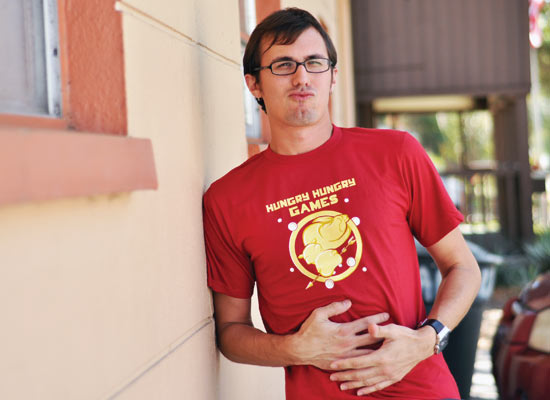
\includegraphics[height=4cm,width=4.5cm]{images/hungrystudent.jpg}
  \ \ \ \ \ \ \ \ \ \ \ \ 
  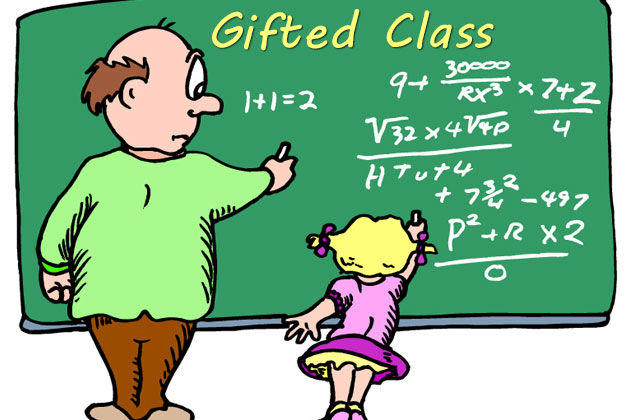
\includegraphics[height=4cm,width=4.5cm]{images/busyprofessor.jpg}
\end{block} 
\begin{itemize}
 \item How to skip the long queue.
 \item How could know Today's menu.
 \item Appropriate menu for me(calorie, price).
 \item Collaborate and share feeling.
 \item How technology can help.
 \end{itemize}
% \framebreak
% 
% \begin{block}{Busy Professors}
%   
\includegraphics[height=1.5cm,width=1.5cm]{images/smartcampuslab.png}
% 
% \end{block} 

\end{frame}

\subsection{Objective}
% \begin{frame}[allowframebreaks]\frametitle{Objective}
\begin{frame}\frametitle{Objective}
Services:
\begin{itemize}
 \item  Mensa Queue Skipper.
 \item  Menu Finder.
 \item  Menu Suggester and Dieting Adviser.
 \item  Customized Menu creator.
 \item  Lunch with Friends.
 \end{itemize}

System should:
\begin{itemize}
 \item  Provide online cafeteria services.
 \item  Provide dieting services to the students.
 \item  Provide social collaboration services.
 \end{itemize}
\end{frame}

\subsection{Proposed Solution}
\begin{frame}\frametitle{Proposed Solution}
\begin{block}{Create ``Smart Cafeteria''}
supported by
\begin{itemize}
 \item web 2.0 system
 \item Smartphone application.
 \end{itemize}
 \end{block}

\begin{block}{``Smart Cafeteria''}
application should be
\begin{itemize}
 \item Interactive.
 \item Adaptive.
 \end{itemize}
 \end{block}
\end{frame}


\section[Analysis]{Analysis}
\subsection{Stakeholders}
\begin{frame}\frametitle{Stakeholders}
\begin{block}{Stakeholders}
 \begin{itemize}
 \item  System Users.
 \begin{itemize}
 \item  Students.
 \item  Professors.
 \item  Researchers.
 \item  University�s Administration Officer.
 \item  University�s Technical Staff.
 \end{itemize}
 \item  System Administrator.
  \begin{itemize}
 \item  Cafeteria Staffs.
 \end{itemize}
 \end{itemize}
  \end{block}
\end{frame}

\subsection{Functional \& Non Functional Requirements}
\begin{frame}\frametitle{Functional \& Non Functional Requirements}
\begin{block}{Functional \& Non Functional Requirements}
Functional Requirements
  \begin{itemize}
 \item  42 Functional Requirements
 \end{itemize}
Non Functional Requirements
 \begin{itemize}
 \item  Usability.
 \item  Internationalization.
 \item  Portability.
 \item  Adaptability.
 \item  Safety and security.
 \end{itemize}
  
\end{block}


\end{frame}

\subsection{Data Gathering \& More Requirements }
\begin{frame}\frametitle{Data Gathering \& More Requirements}
\begin{block}{Data Gathering \& More Requirements}
 \begin{itemize}
 \item  Focus Group - 7 participants.
 \item  Questionnaires.
 \end{itemize}
\end{block}
\begin{block}{Outcomes}
 \begin{itemize}
 \item ``Smart Cafeteria'' is usefull application.
 \item Found 5 more functional requirement.
 \item Design UML (4 Use Case, Class Diagram, 4 Activity Diagram.)
 \end{itemize}
\end{block}
\end{frame}

\section[Design]{Design}
\subsection{Desktop Prototype}

\begin{frame}\frametitle[allowframebreaks]{Desktop Prototype[Index Page]}

\centering
  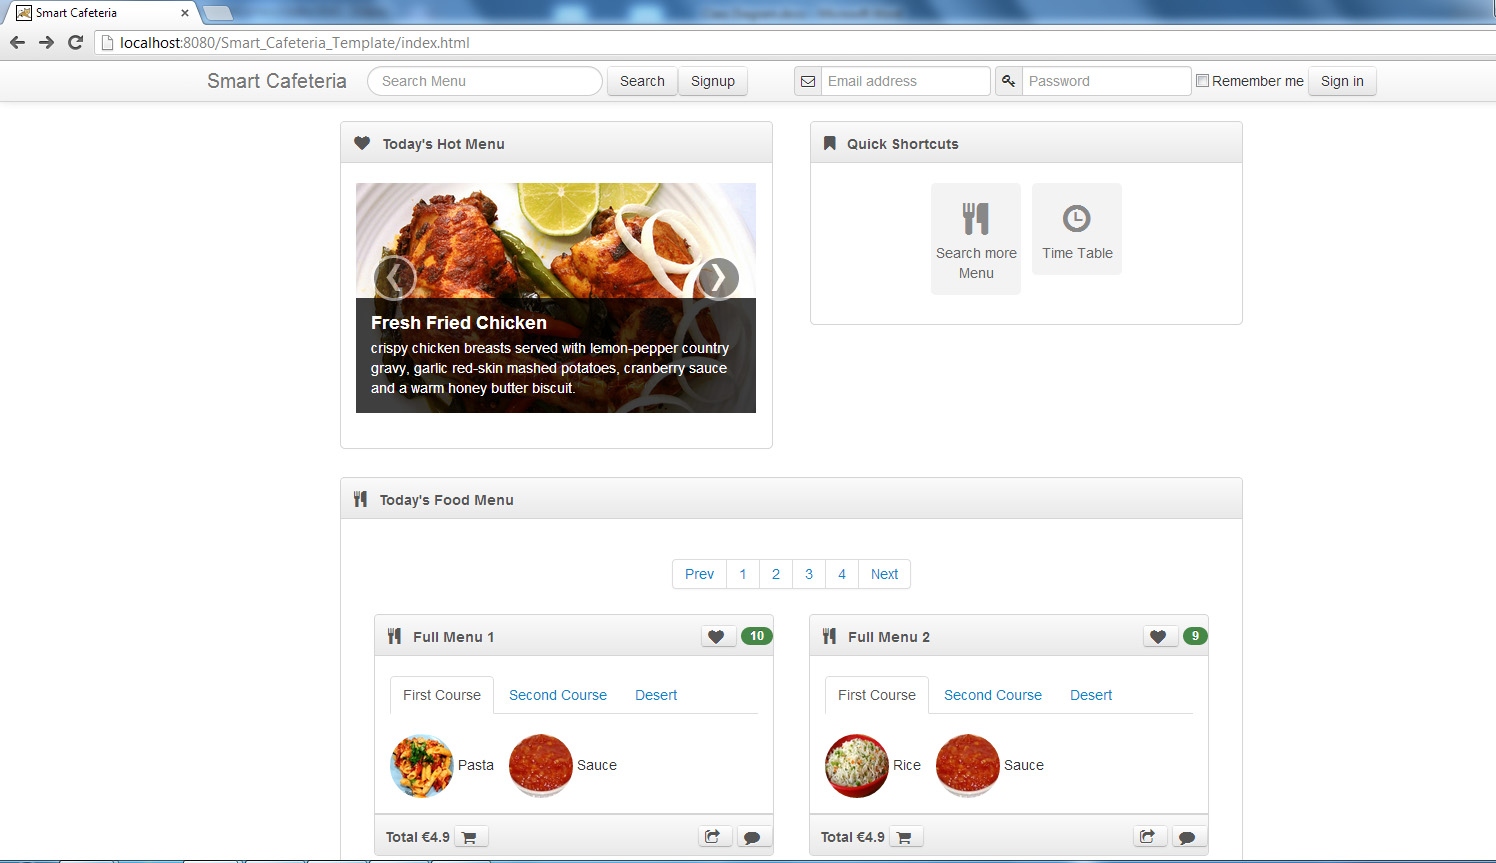
\includegraphics[height=6cm,width=10cm]{images/index.jpg}

\end{frame}

\framebreak
\begin{frame}\frametitle{Desktop Prototype[User Dashboard]}

\centering
  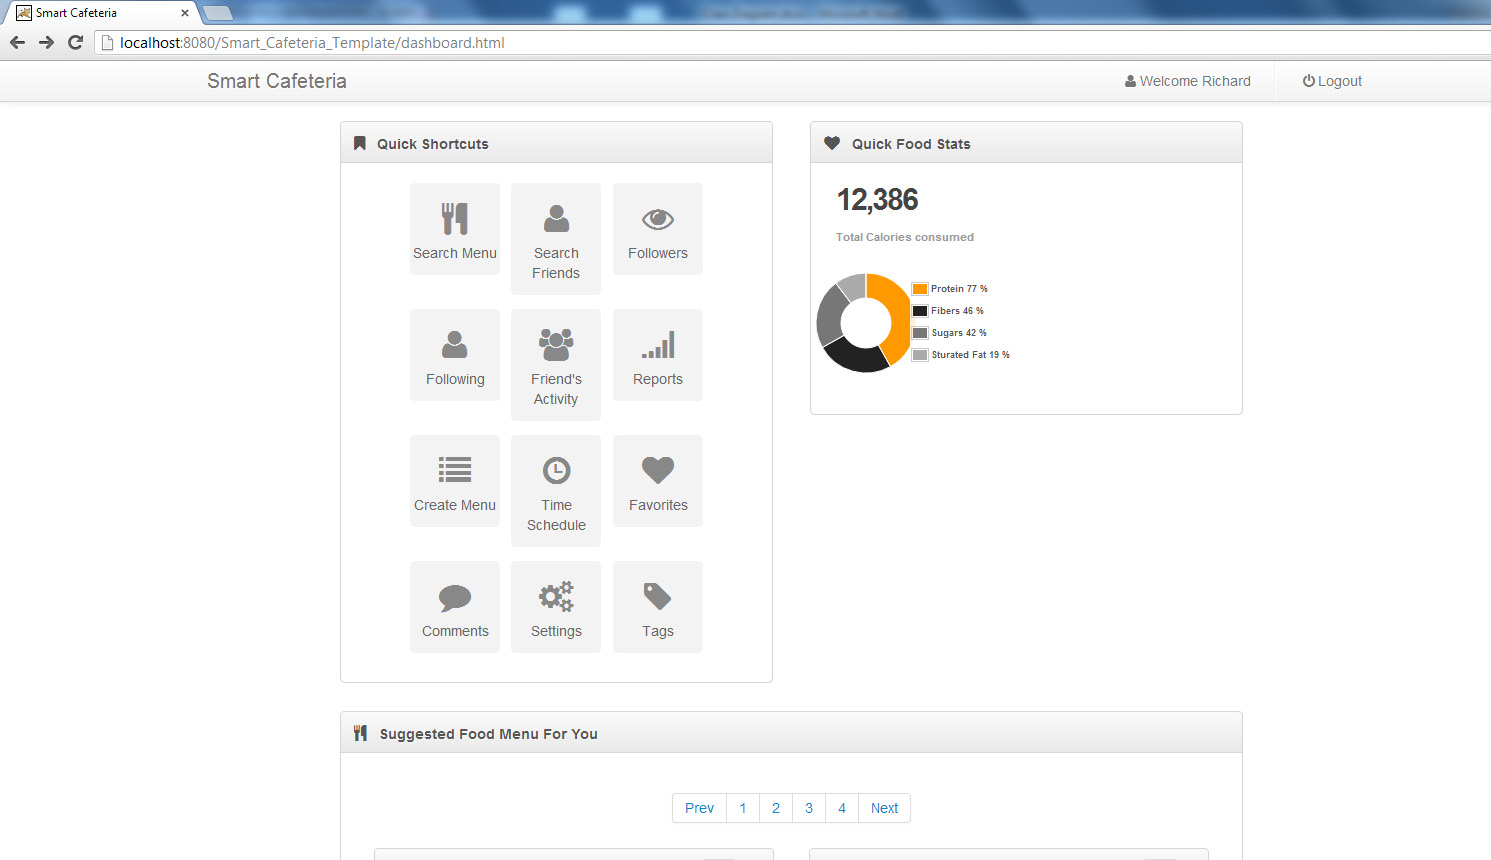
\includegraphics[height=6cm,width=10cm]{images/dashboard.jpg}

\end{frame}

\framebreak
\begin{frame}\frametitle{Desktop Prototype[Suggested Food Menu]}

\centering
  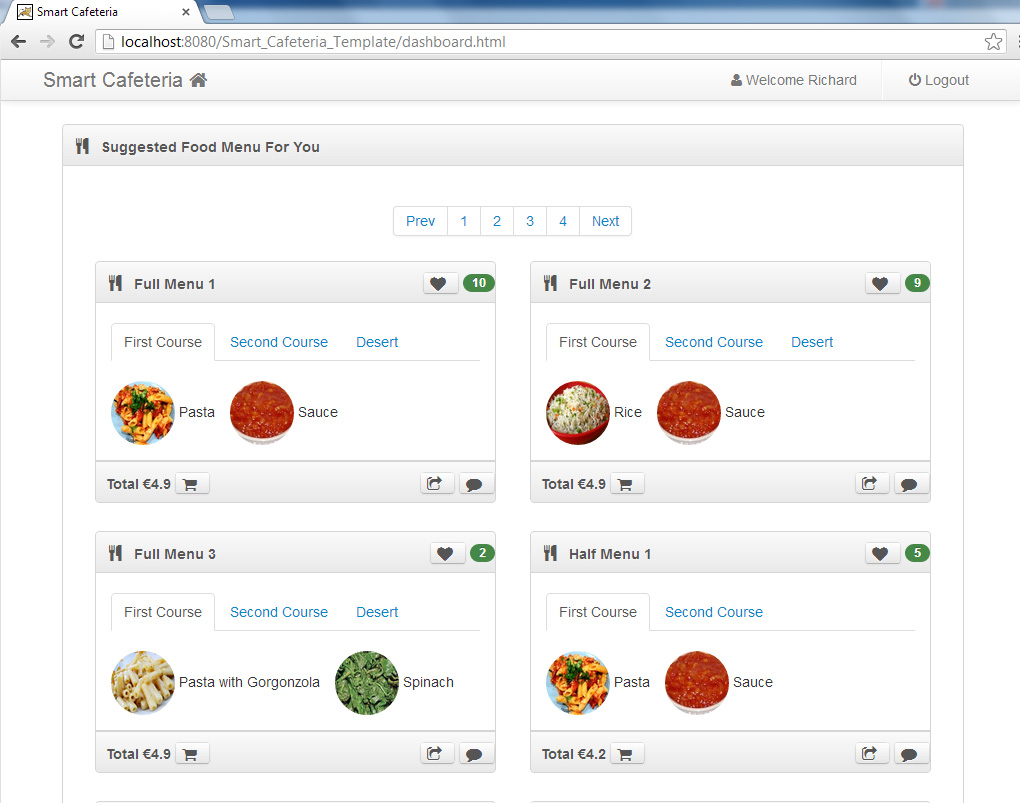
\includegraphics[height=6cm,width=10cm]{images/foodmenusuggestion.jpg}

\end{frame}
\subsection{Mobile Prototype}
\begin{frame}\frametitle{Mobile Prototype}
 \centering 
  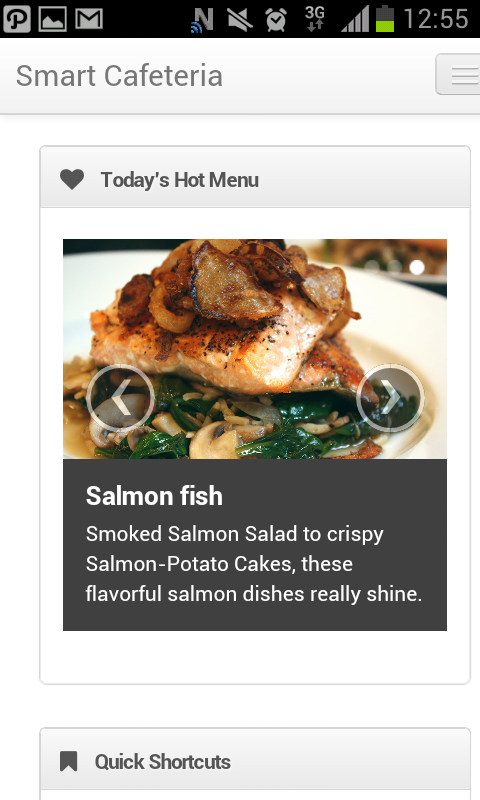
\includegraphics[height=6cm,width=4cm]{images/mobile-index.png}
   \ \ \ \ \ \ 
  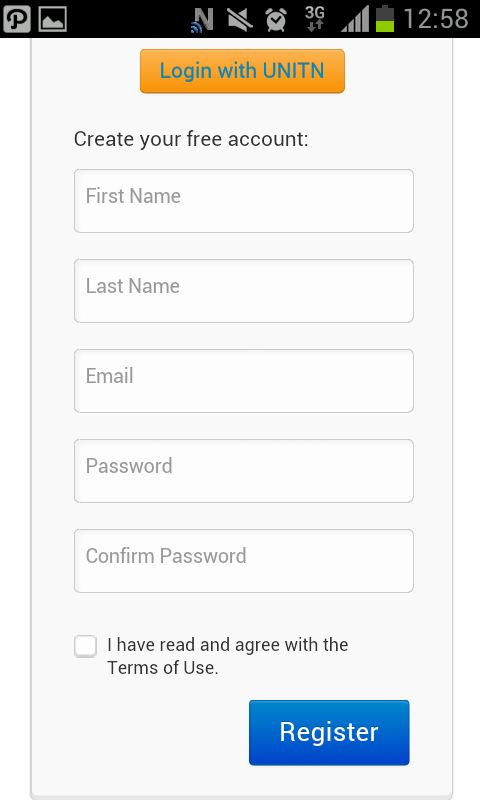
\includegraphics[height=6cm,width=4cm]{images/mobile-registration-step1.png}
  %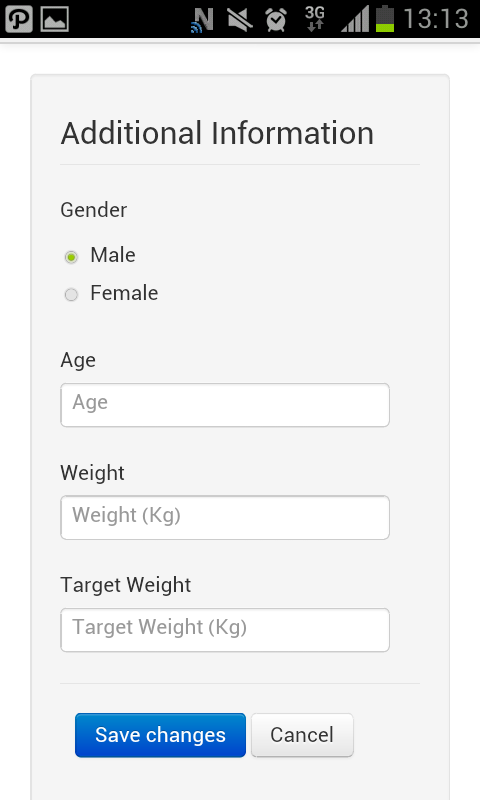
\includegraphics[height=6cm,width=4cm]{images/mobile-registration-step2.png}

\end{frame}

% \subsection{Features of Smart Cafeteria Design}
% \begin{frame}\frametitle{Features of Smart Cafeteria Design}
% Key Features of Smart Cafeteria Design
%  \begin{itemize}
%  \item Online Cafeteria services.
%  \item Adaptive services.
%  \item Social collaboration services.
%  \item Mobile Interaction.
%  \end{itemize}
% 
% \end{frame}

\section[Evaluation]{Usability Evaluation}
\subsection{Evaluation Methodology}
\begin{frame}\frametitle{Evaluation Methodology}
 \begin{itemize}
   \item Evaluation Methodology: User studies and questionnaire.
   \item 10 participants.
   \item Given them 9 tasks to perform.
   \item Given them 14 usability questions [likert scale: 1-7] to test.
 \begin{itemize}
    \item usefulness
    \item easy to use
    \item learnability
    \item Satisfaction
\end{itemize}
	\item Evaluation for Desktop and Mobile Prototype.
	\item Calculate Mean($\mu$) and Standard deviation($\sigma$)\\
	$\sigma$ =  $\sqrt{\frac{1}{N}\sum_{i}^{N} (x_i - \mu^2)} $ \\
	$\mu$ = $\frac{1}{N}\sum_{i}^{N} x_i$.
\end{itemize}
\end{frame}

\subsection{Evaluation Result}
\begin{frame}\frametitle{Result for desktop Prototye}
\centering
  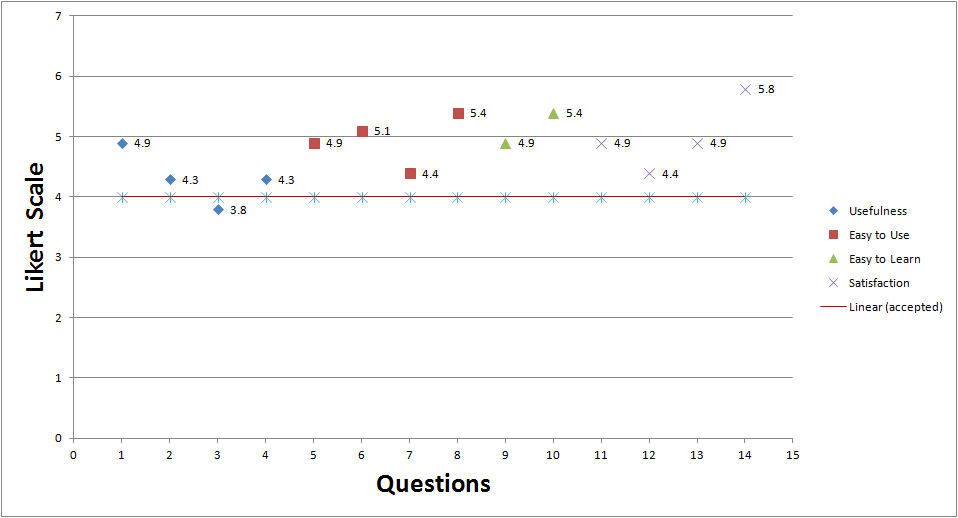
\includegraphics[height=6cm,width=10cm]{images/UsabilityEvaluationGraphDesktop.jpg}

\end{frame}
\begin{frame}\frametitle{Result for Mobile Prototye}
\centering
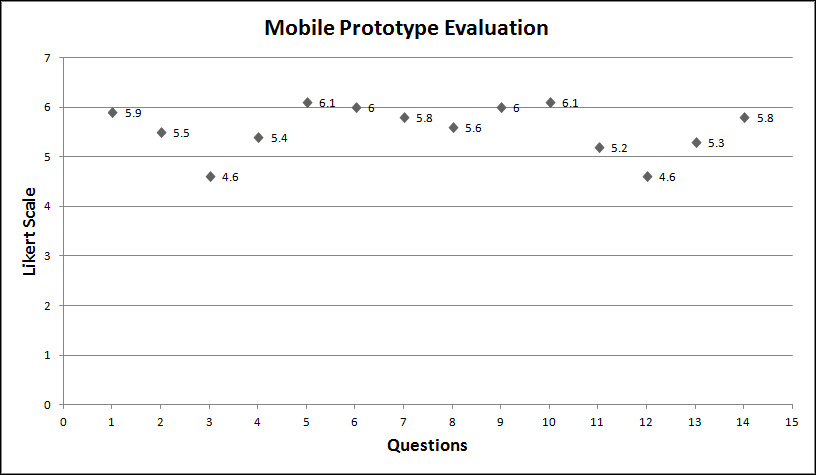
\includegraphics[height=6cm,width=10cm]{images/UsabilityEvaluationGraphMobile.jpg}
\end{frame}

\section[Conclusion]{Conclusion}

%\subsection{Conclusion and Future Work}

\begin{frame}\frametitle{Conclusion and Future Work}
``Smart Cafeteria''
 \begin{itemize}
    \item Could solve the problems mostly [reduce queue time].
    \item is adaptive [its functionalities].
    \item is interactive [usability].
\end{itemize}
Future Work
 \begin{itemize}
    \item Build high fidelity prototype [full functional]. 
    \item Find best machine learning approach for adaptability.
    \item More User Study for better usability.
\end{itemize}
\ \\
Resources 
 \begin{itemize}
    \item Github Repository \url{https://github.com/suptaphilip/Master-Thesis}
    %\item Github Page \url{http://suptaphilip.github.io/Master-Thesis/}
\end{itemize}
\end{frame}

%\subsection{Questions}
\begin{frame}\frametitle{Questions}
\begin{center}
\textbf{\textsc{Any Questions}} \\

\includegraphics[height=4cm,width=4cm]{images/question.jpg} \\
\textbf{Thanks}
\end{center}

\end{frame}

\end{document}